\section{Testing and Observations}
\label{section:testing_and_observations}
\subsection{Keypad Debouncing}
Our first component that required testing was the keypad, which unfortunately did not have a formal datasheet available. An important required step for us to figure out which output pin was set by the buttons on the keypad. Our approach to debugging this was to connect what was presumed to be the column pins to the digit pins of the display, and then to press the buttons and observe which segment would light up. Once the keypad pins were mapped and each button was assigned a combination of COL and ROW pins, our focus shifted towards debouncing the digit presses. This was achieved using a deboucing interval of 200ms, in combination with a minimum update count, which is described in Section \ref{section:implementation}. During testing, we observed that this debouncing mechanism worked without problems. %Furthermore, to enter consecutive numbers the user would need to press a second time with a 200ms pause between presses to let the controller know that the button had been released character is pressed and a consecutive repeating character is a new character and not a continuation of the initial digit press.

\subsection{ADC Thread}
We initially implemented an additional thread for our ADC that would wake up as soon as the \verb|DMA_buffer_full()| callback was executed by setting a flag. This through testing however showed that the ADC thread would end up blocking the other threads from executing and eventually block our whole program. Figure ? bellow shows our program output and shows the display and keypad threads getting called until only the ADC thread output is shown.



\begin{figure}[h]
\centering
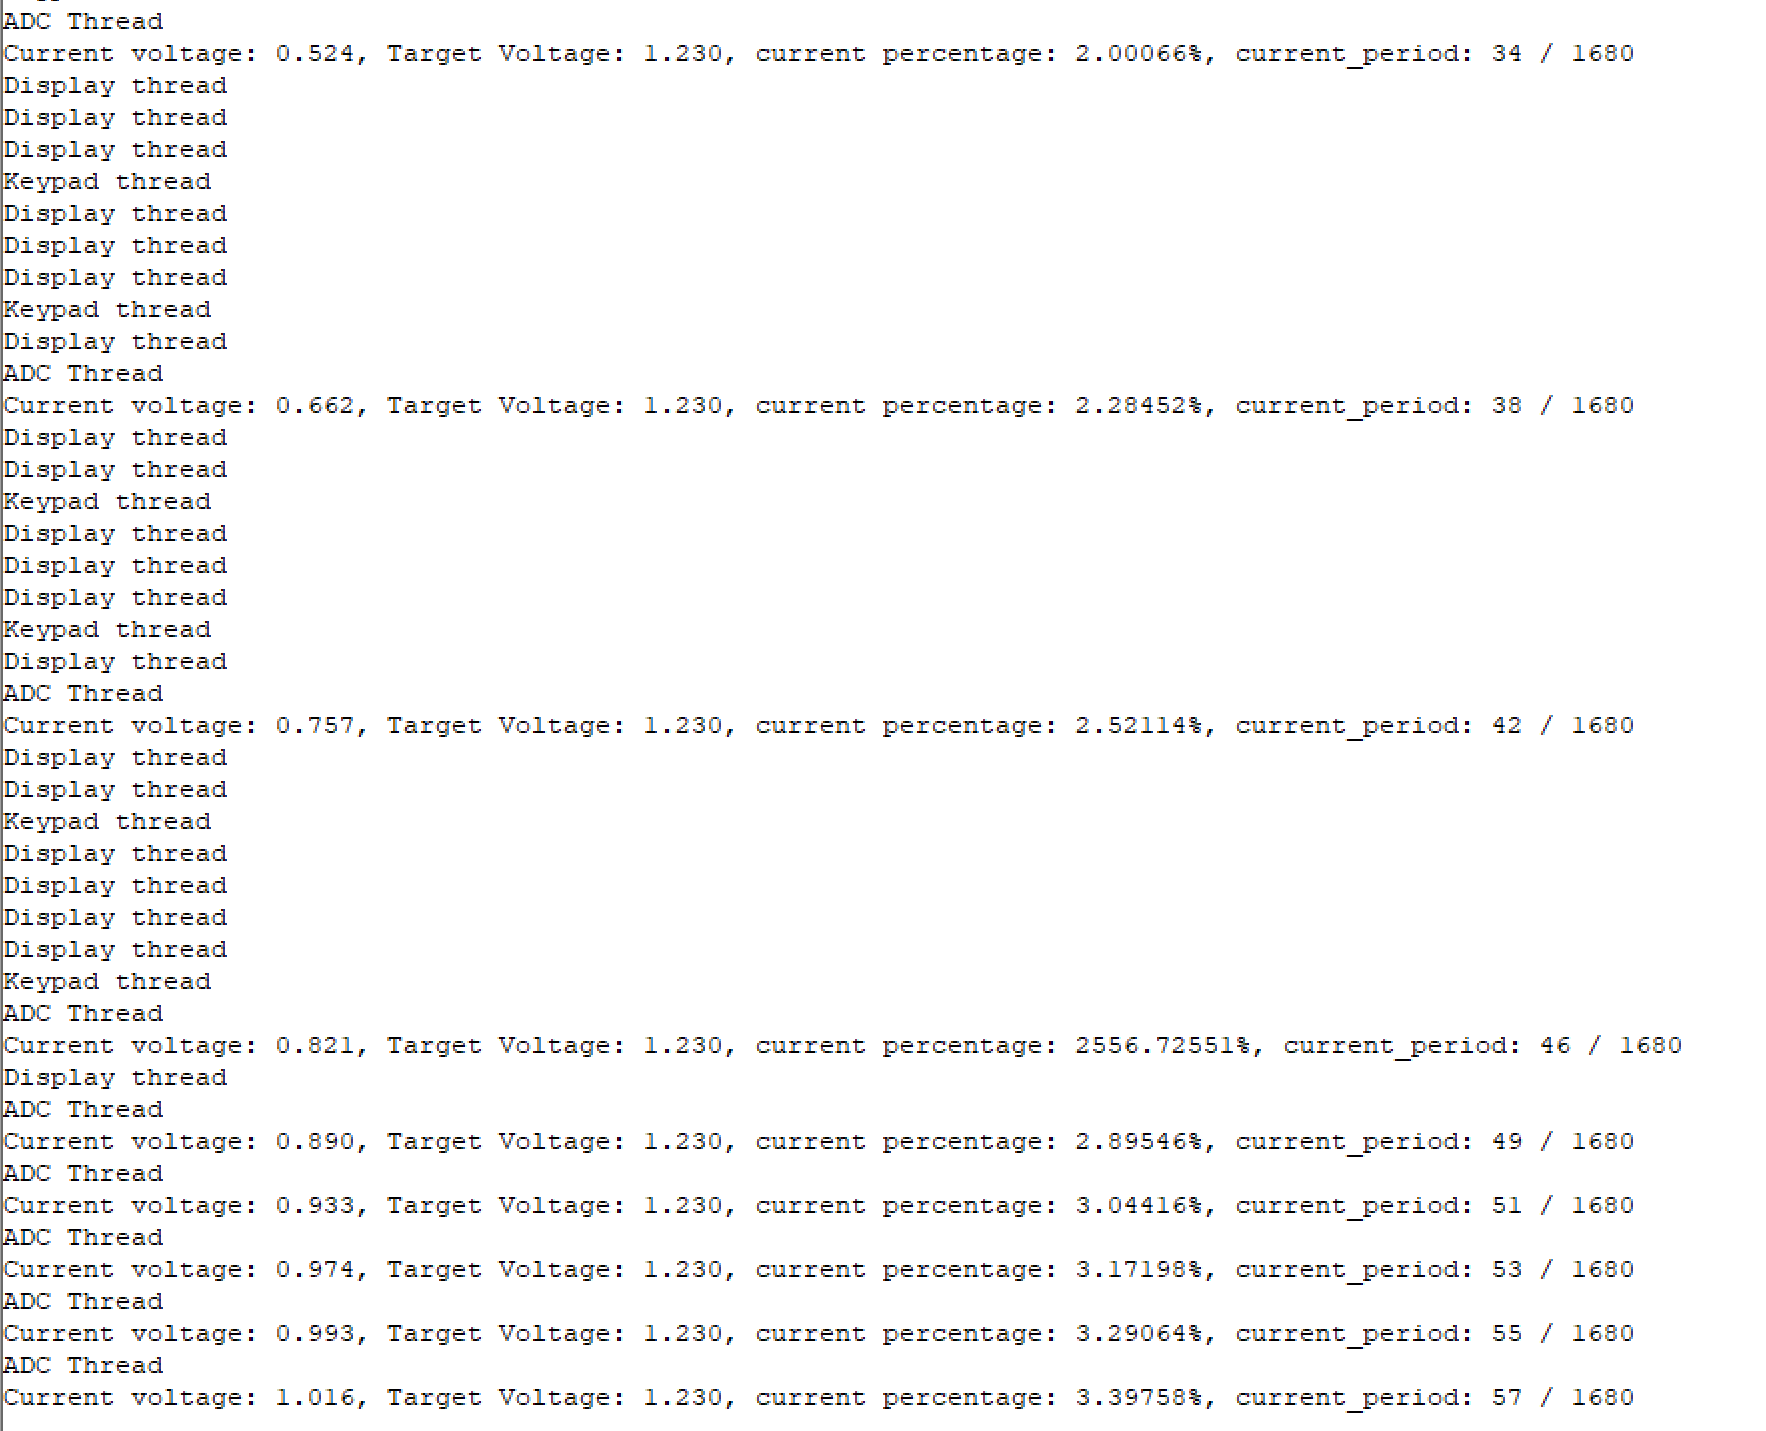
\includegraphics[scale=0.5]{images/weird_behaviour.png}
\caption{
\label{fig:weird_behaviour}
An example of the very weird behaviour observed when using an ADC thread. The ADC, Keypad and Display threads are coexisting peacefully, up until the point at which the ADC thread decides it will keep the CPU all for itself.
}
\end{figure}





To overcome this blocking thread we decided to just keep our ADC DMA processing in a service routine called after every full buffer callback instead of relying on raising the flag to wake up the ADC thread. With this implementation the keypad and display threads would work properly without the blocking that previously occurred.
The next component to test was our PWM wave generated by timer 3. We connected the oscilloscope to the positive terminal of the diode and plotted the wave form. Seen in Figure \ref{fig:PWM_duty_cycle} we can see that our duty cycle was around %$25%$ and 

\begin{figure}[h]
\centering
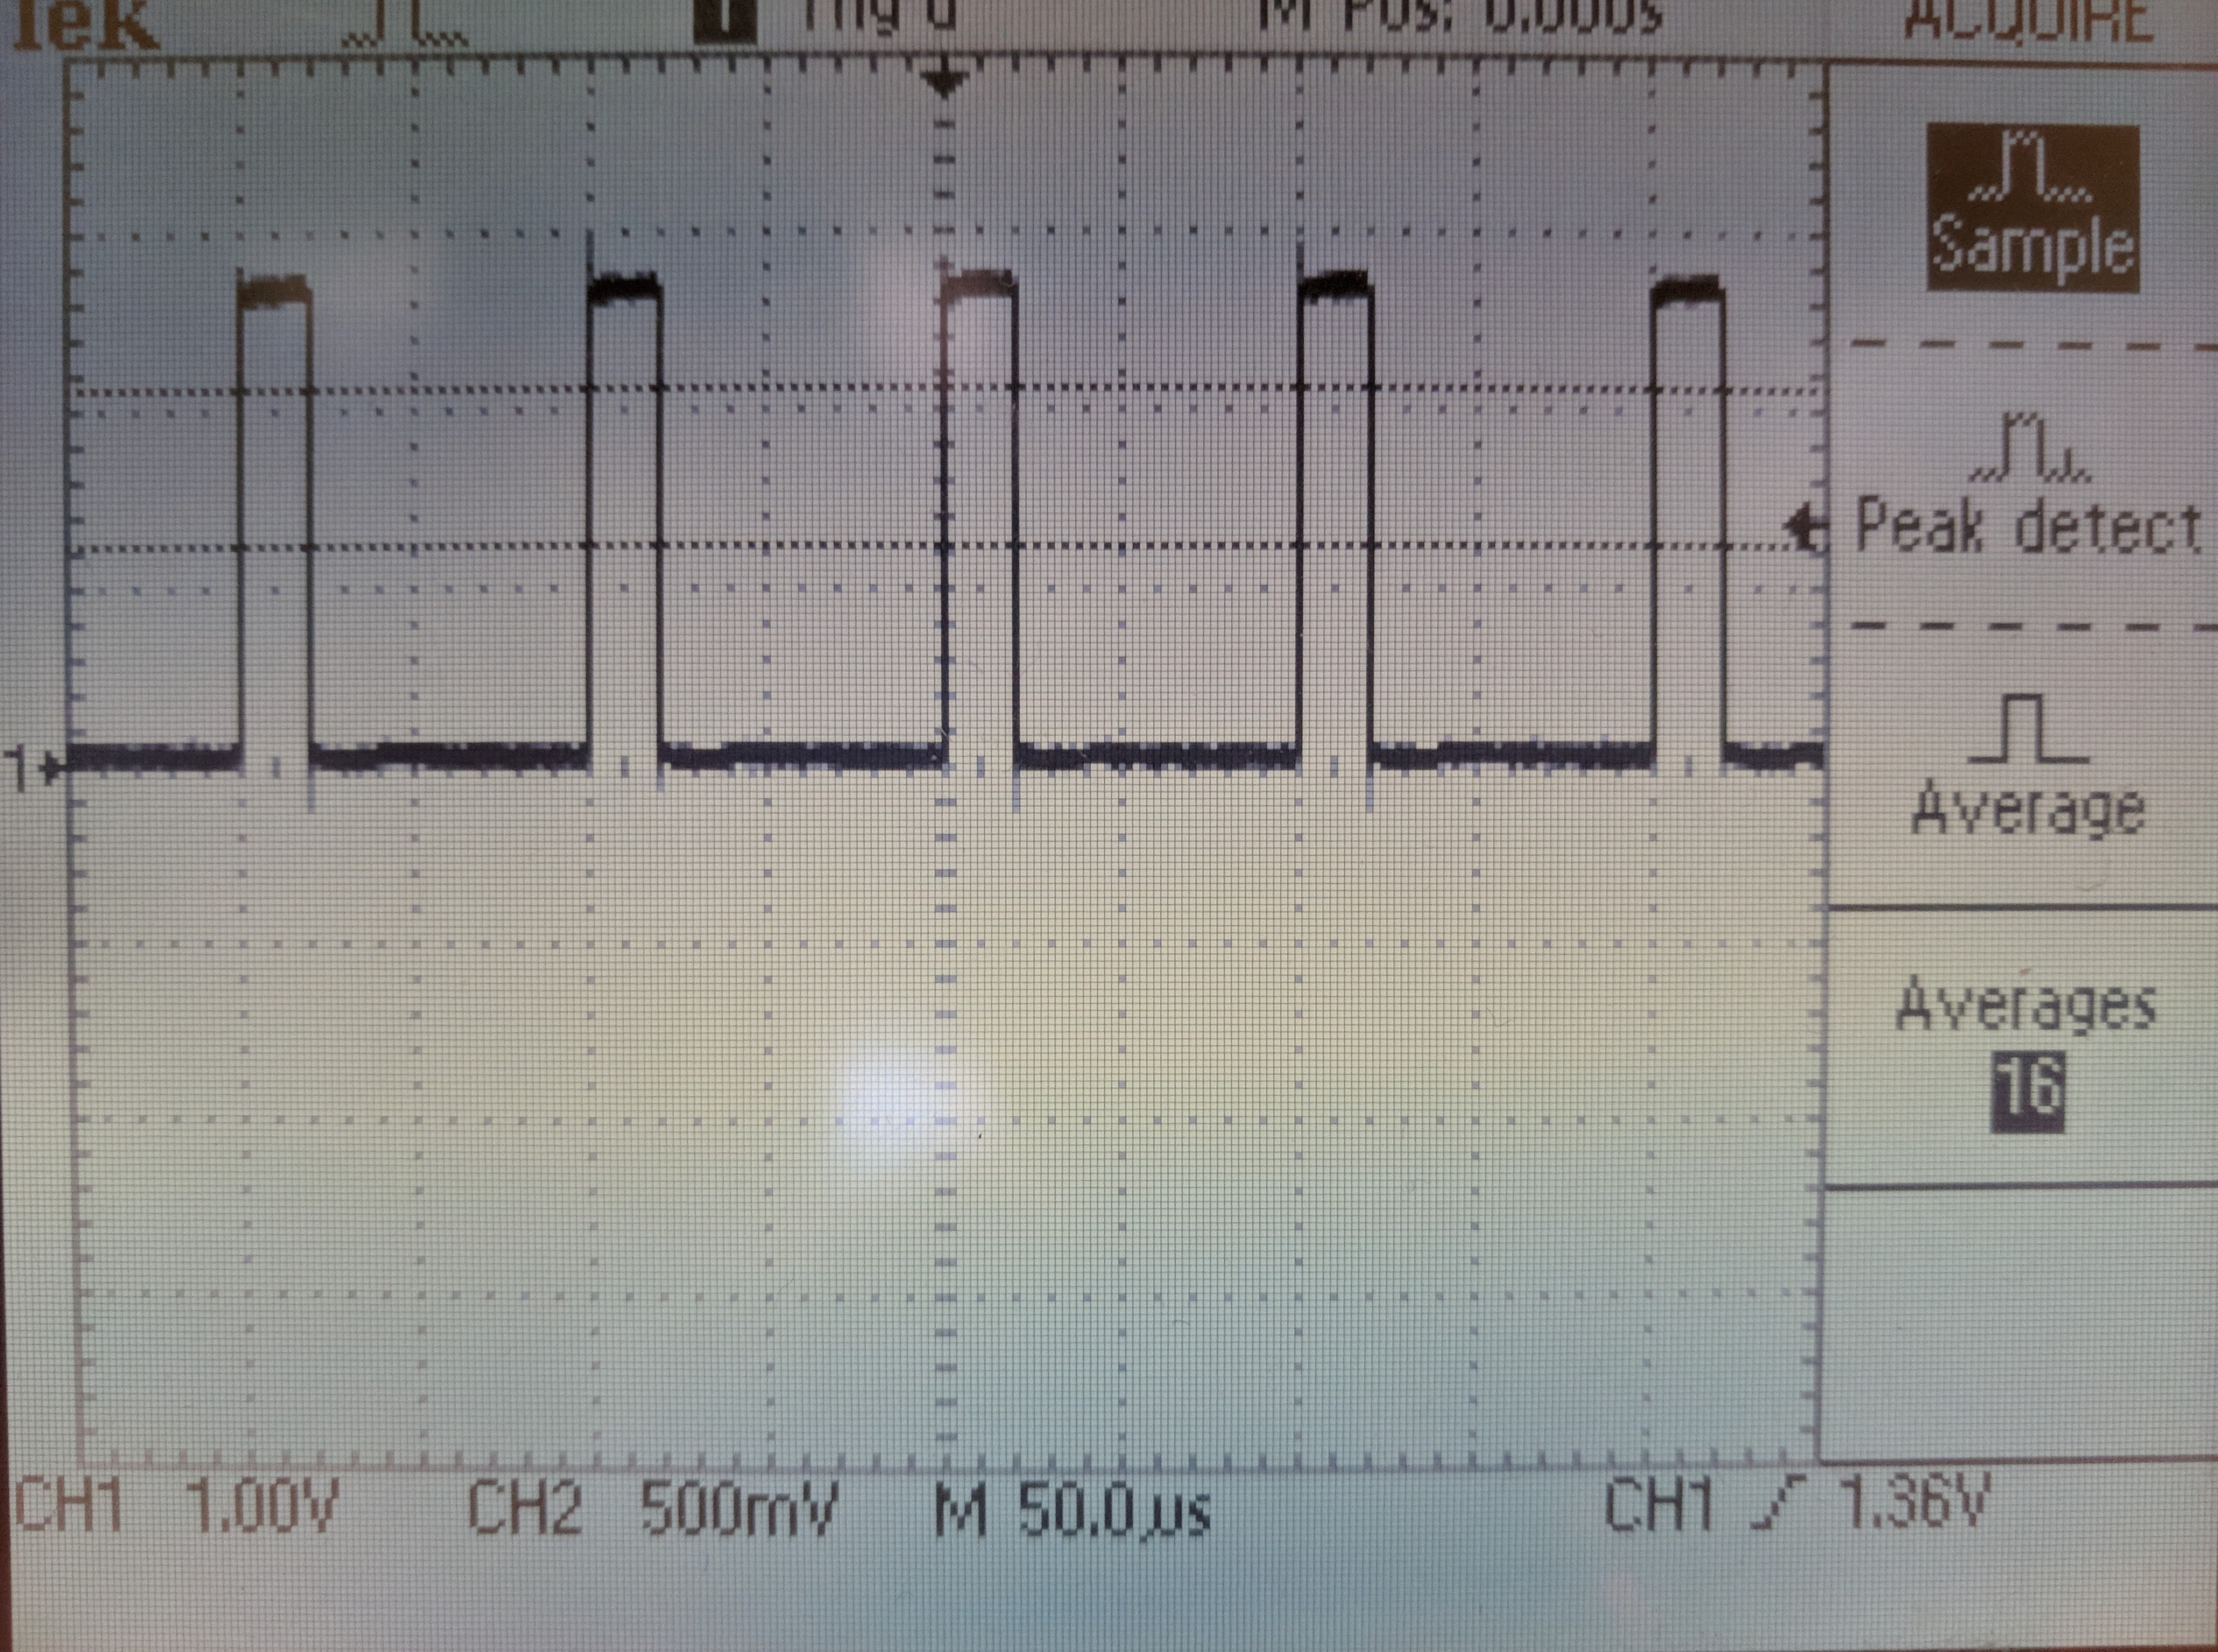
\includegraphics[scale=0.1]{images/pwm_duty_cycle.jpg}
\caption{\label{fig:PWM_duty_cycle} Sample of the PWM signal.}
\end{figure}


Our first controlled was modified from the idea introduced in the Theory and Hypothesis and can be seen working in Figure ?. Because this controller adjusts the duty cycle based off of the difference between measured and target RMS values, it doesn't reach the target RMS value near the end of the adjustments.
\todo[inline]{first Controller picture HERE}




In contrasts to the first implemented controller our second one uses a Binary Search approach that tends to overshoot and re-correct as seen in Figure ?. Although this controller is much faster than our first one, it does overshoot which may not be ideal depending on the direct implementation this controller may be used in. For the purposes of this project is it adequate.
\todo[inline]{second Controller picture HERE}
